\chapter{Stand der Technik}
\label{chap:standTechnik}
Dieses Kapitel soll ein grundlegendes Verständnis wiedergeben, wie der momentane Stand der
Technik aussieht. Dabei soll zunächst betrachtet werden, wie die
momentane Entwicklung bei eingebetteten Systeme vonstattengeht, um anschließend eine
beispielhafte Anwendung zu implementieren. Zudem soll auch das Framework dieser Thesis
vorgestellt werden.
\section{Embedded Systems}
\label{sec:EmbeddedSystems}
Ein Embedded System oder auf Deutsch ein eingebettetes System wird als eine integrierte,
mikroelektronische Steuerung angesehen. Welches meist darauf ausgelegt ist eine spezifische Aufgabe
zu erledigen \cite{EmbeddedSystem}[vgl.]. Dabei setzt sich ein Embedded System aus dem
Zusammenspiel zwischen
Hardware und Software zusammen. Solche Embedded Systems haben meist kein ausgeprägtes
Benutzerinterface und können weitergehend in die zwei Unterklassen, Non-Deeply und Deeply Embedded
Systems unterteilt werden.
\newline
\newline
Neben der logischen Korrektheit, die Embedded Systeme erfüllen müssen, lassen sie sich
durch eine Reihe unterschiedlicher Anforderungen und Eigenschaften von den heutzutage üblichen
Anwedungen abgrenzen. Unter anderem werden bei Embedded Systems ein sogenanntes
\emph{Instant on} gefordert, welches besagt, dass das Gerät unmittelbar nach dem Einschalten
betriebsbereit sein muss \cite{EmbeddedLinuxQuade}[vgl.].
\newline
\newline
Folgende Tabelle zeigt die typischen Anforderungen an ein Embedded System auf:

\begin{table}[ht]
    \centering
    \begin{tabularx}{\textwidth}{md}
        \textbf{Anforderung} & \textbf{Beschreibung}                                           \\
        \hline
        Funktionalität   & Die Software muss schnell und korrekt sein
        \\\rowcolor{Gray}
        Preis           & Die Hardware darf nicht zu kostspielig sein                 \\
        Robustheit       & Muss auch in einem rauen Umfeld funktionieren
        \\\rowcolor{Gray}
        Fast poweroff     & Muss in der Lage sein schnell das komplette System abzuschalten   \\
        Räumliche Ausmaße  & Muss klein sein, um sich in ein System einbinden zu können
        \\\rowcolor{Gray}
        Nonstop-Betrieb   & Muss in der Lage sein, im Dauerbetrieb laufen zu können          \\
        Lange Lebensdauer  & Muss in der Lage sein, teilweise mehr als 30 Jahre zu laufen
    \end{tabularx}
    \caption[Anforderungen an Embedded Systems]{Anforderungen an Embedded Systems
    \cite{EmbeddedLinuxQuade}}
    \label{table:AnforderungenEingebetteteSysteme}
\end{table}

\subsection{Hardware}
\label{subsec:EmbeddedHardware}
Test
\subsection{Software}
\label{subsec:EmbeddedSoftware}
Genauso wie sich Embedded Systems in zwei Bereiche unterscheiden lassen können, kann die
Software eines Embedded System in Systemsoftware und funktionsbestimmende
Anwendungssoftware unterteilt werden.
Für ein \emph{Deeply Embedded System} wird in den meisten fällen ein Echtzeitbetriebssystem
(Realtime Operating System - RTOS) verwendet, welches an die Hardware angepasst ist.
\newline
\newline
Ganz anders sieht es im \emph{Non-Deeply Embedded Systems} Bereich aus. Da diese für sehr
komplexe Aufgaben zum Einsatz kommen, kommt es nicht selten
vor, dass eine \ac{gui} für ein solches System vonnöten ist. Deswegen basiert ein
\emph{Non-Deeply
Embedded Systems} auf einer Systemsoftware, die Programmierer*innen mehr Möglichkeiten bei
der Entwicklung geben. Unter anderem ist die Möglichkeit gegeben, die Programmiersprache
und
das \ac{gui}-Framework selbst auszusuchen \cite{EmbeddedLinuxQuade}[vgl.].

\section{Qt}
\label{sec:qt}
In der vorherigen Sektion wurde ein allgemeines Bild dargestellt, was ein eingebettetes System
ist und in welchen Varianten diese auftauchen. Weitergehend soll nun, in dieser Sektion,
vorgestellt werden, mit dem üblicherweise im \emph{Open Embedded Systems} bereich programmiert wird.
\newline
\newline
Ein großer Anteil eines \emph{Open Embedded Systems} wird heutzutage durch die \ac{gui}
repräsentiert. Die \ac{gui} sollte intuitive und zuverlässig sein.
Zudem ist es auch noch enorm wichtig, dass die \ac{gui} wenige Resourcen verbraucht, schnell
reagiert und einfach einzubinden ist. Um diese Anforderung zu erreichen, wurde bis Dato \emph{Qt} in
Kombination mit der Programmiersprache \emph{C++} verwendet \cite{QtOnEmbeddedLinux}[vgl.].

\subsection{Was ist Qt?}
\label{subsec:WasIstQt}
Qt ist ein Framework zum Erzeugen von GUIs auf mehreren Betriebssystemen. Es wurde 1990 von
\emph{Haarvard Nord} und \emph{Eirik Chambe-Eng} mit dem entwickelt, benutzerfreundliche GUIs
mithilfe
der Programmiersprache C++ zu entwickeln. Der Name \emph{Qt}
entstand dabei, da Haarvard den Buchstaben \emph{Q} in Emacs als sehr schön empfand. Zudem
entstand das \emph{t} in Qt als
Abkürzung für das englische Wort \emph{Toolkit} \cite{qtStory}[vgl.].
\newline
\newline
Weitergehend sollte mit Qt die Möglichkeit geschaffen werden, mit nur einer Code-basis alle
Betriebssysteme abzudecken. Die schwierigkeit bestand also darin, das selbe Aussehen
und die gleiche Funktionalität über die verschiedenen Betriebssysteme zu
schaffen \cite{GettingStartedQt}[vgl.].
\newline
\newline
Qt ist in C++ entwickelt worden und verwendet zusätzlich noch einen Compiler welcher
\emph{\ac{moc}} genannt wird, womit C++ um weitere Elemente erweitert wird. Der daraus
compilierte Code folgt dem C++-Standard und ist somit mit jedem anderen C++ Compiler kompatibel.
Obwohl Qt ursprünglich dafür gedacht war, rein auf C++ zu basieren, wurden im Laufe der Zeit
mehrere Eweiterungen für Qt von der Community entwickelt, um Qt mit mehreren Programmiersprachen
benutzen zu können, wie zum Beispiel Python oder Java.
\begin{figure}[h]
    \centering
    
\includegraphics[width=0.4\textwidth, center]{StandDerTechnik/qtLogo}
    \caption[Qt Logo]{Qt Logo}
    \label{img:qtLogo}
\end{figure}
\subsection{Programmierbeispiel}
\label{subsec:programmierbeispiel}
Das Programmierbeispiel welches im Folgenden dargestellt wird, erzeugt ein Fenster mit dem Titel 
\emph{Meine erste Qt App}. Zudem ein Label welches \emph{Hello World} anzeigt und ein Button mit der
Aufschrift \emph{Exit}. Sobald der Button wird, schließt sich das Fenster.

\lstinputlisting[language=C++,caption={Qt Hello World Sourcecode},
    label=lst:qtHelloWorldSourceCode]{\srcloc/StandDerTechnik/qtHelloWorld.cpp}

Daraus ergibt sich das folgende Programm
\begin{figure}[h]
    \centering
    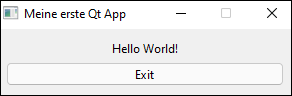
\includegraphics[width=0.5\textwidth, center]{StandDerTechnik/qtHelloWorldApp1}
    \caption[Qt Hello World App]{Qt Hello World App}
    \label{img:qtHelloWorldApp}
\end{figure}
\subsection{Widgets}
\label{subsec:widgets}
Um eine \ac{gui} gestalten zu können braucht es Komponenten, die auf der \ac{gui} angezeigt
werden können. Qt verwendet dafür sogenannte \emph{Widgets}. Widgets sind also grafische
Komponenten, die dafür genutzt werden können, um die Benutzeroberfläche nach belieben zu
gestalten. Ein Beispiel für eine solche Komponente wäre ein Button, welcher in der Sektion
\emph{\nameref{subsec:programmierbeispiel}} als \emph{btnExit} vorkam.
\newline
\newline
Die Widgets, die Qt zur verfügung stellt sind in einer großen Klassenhierarchie zusammengesetzt
und diese Hierarchie könnte sich wie folgt vorgestellt werden:

\begin{figure}[h]
    \centering
    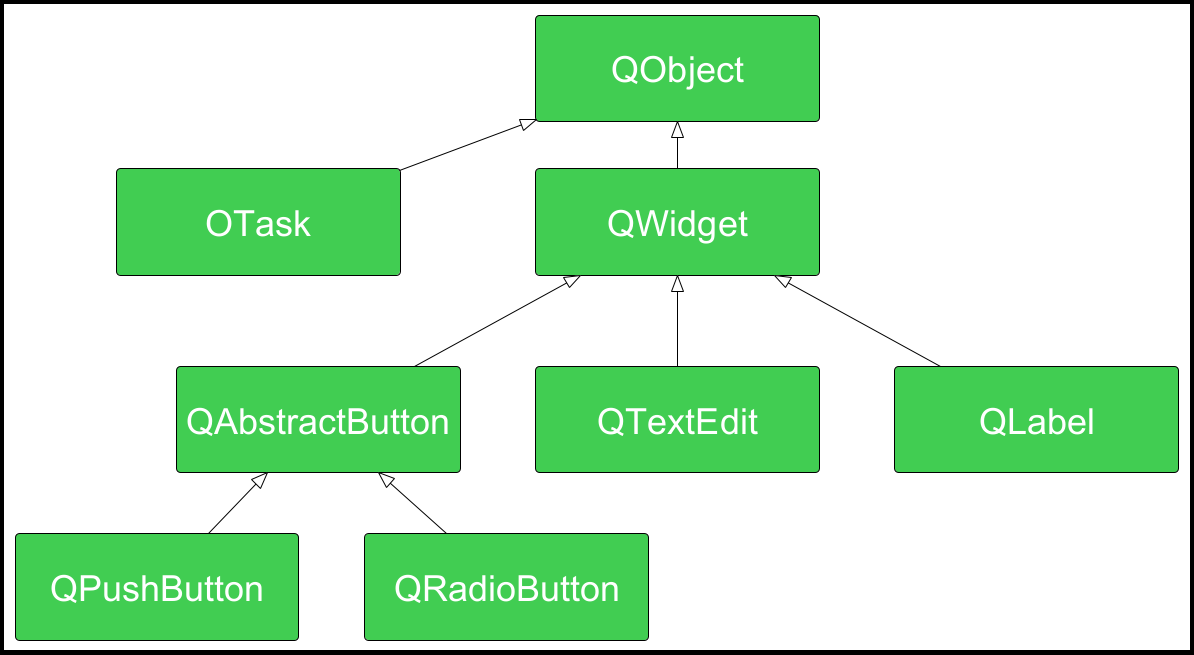
\includegraphics[width=\textwidth, center]{StandDerTechnik/qtWidgetClassHierachie}
    \caption[Qt Widgets Klassenhierachie]{Qt Widgets Klassenhierarchie
    \cite{GettingStartedQt}[vgl.]}
    \label{img:qtWidgetClassHierachie}
\end{figure}

Wie zu sehen ist, ist ganz oben in der Klassenhierarchie die \emph{QObject} Klasse. Diese
enthällt unter anderem den Signal und Slot mechanismus, welcher später noch genau erklärt wird.
Weitergehend, werden Widgets, die gemeinsame Funktionalitäten aufweisen zusammen grupiert. Diese
Verhalten ist bei \emph{QPushButton} und \emph{QRadioButton} erkennbar, denn beide Widgets sind
Buttons, die sich Teilweise die gleichen Eigenschaften und Funktionen teilen
\cite{GettingStartedQt}[vgl.].

\subsection{Signal und Slot Konzept}
\label{subsec:signalslot}
Eine interaktive Benutzeroberfläche muss auf
Ereignisse reagieren können. Beispielsweise ist das Betätigen eines Buttons ein Auslöser für ein
Ereignis auf welches reagiert werden kann. Es gibt viele Methoden und Muster in welche ein
solches Ereignis-Aktionskonzept implementiert werden kann.

Ein \emph{Signal} ist im einfachen Sinne eine Nachricht, die versendet werden kann. Die Nachricht
signalisiert, dass sich der momentane Status eines Objektes geändert hat. Dahingegen ist ein
\emph{Slot} eine spezielle Funktion von einem Objekt, welche dann aufgerufen wird, wenn ein
bestimmtes \emph{Signal} gesendet wird \cite{GettingStartedQt}[vgl.].

Damit jeder \emph{Slot} auch weiß, auf welches \emph{Signal} reagiert werden soll, müssen diese verbunden werden. In der Sektion \emph{\nameref{subsec:programmierbeispiel}} war
folgende Zeile zu sehen:
\newpage
\begin{lstlisting}[language=C++, caption=Signal- und Slot-Beispiel, label=lst:SignalSlotBeispiel]
// Connect button with the App
QObject::connect(btnExit, SIGNAL(clicked()), &app, SLOT(quit()));

\end{lstlisting}

In dieser Codezeile fand die Verbindung zwischen einem Signal und einem Slot statt.
Wenn der Button betätigt wird, wird \emph{app} signalisiert und ruft \emph{quit()} auf. Die
Funktion \emph{quit()} beendet das Programm.

Einer der größten Vorteile dieser Methode im Gegensatz zu anderen Methoden ist, dass dadurch
n:m-Beziehungen abgebildet werden können. Das bedeutet also, dass sich ein Signal mit
beliebig viel Slots verbinden kann und dass sich ein Slot auf mehrere Signale verbinden kann
\cite{SignalSlotMechanismus}[vgl.].
%\subsection{Raspberry Pi und Qt}
\label{subsec:rasPiUndQt}
Nachde ein grober Überblick zu Qt geschaffen wurde, soll nun eine beispielhafte Anwendung
mithilfe von Qt auf dem Raspberry Pi implementiert werden. Bei dieser Anwendung sollen beim
Betätigen eines Buttons Daten von dem Raspberry Pi gelesen werden und auf der \ac{gui} angezeigt
werden. Dieses Beispiel ist von dem Embedded Systems 2 Labor inspiriert.

\subsubsection{RTIMULib}
\label{subsubsec:RTIMULib}
Die RTIMU Bibliothek war anfändlich dazu gedacht, mithilfe von C++ oder
Python Daten von einem Non-Deeply Embedded System zu lesen. Mitlerweile existiert diese
Bibliothek auch für andere Sprachen wie zum Beispiel C\#.
\newline
\newline
Mithilfe dieser Bibliothek sollen für dieses Beispiel die Daten von dem Raspberry Pi gelesen
werden, um diese dann anschließend auf der \ac{gui} anzeigen zu können. Um RTIMU in einem QT
Projekt nutzen zu können, muss die Bibliothek zunächst in der \emph{.pro} Datei eingebunden
werden. Dies geschieht, indem die Zeile \emph{LIBS += -lRTIMULib} hinzugefügt wird.

\subsubsection{Hilfsklasse}
\label{subsubsec:Hilfsklasse}
Nachdem die Bibliothek hinzugefügt wurde, soll eine Hilfsklasse als Repräsentation der Daten
erzeugt werden. Das folgende Listing zeigt dies auf:

\begin{lstlisting}[language=C++, caption=RTIMU-Hilfsklasse, label=lst:Hilfsklasse]
class ReadData
{
private:
    float m_Temperature = 0.1f;
    float m_AirPressur = 0.1f;
    float m_Humidity = 0.1f;
    float m_xMagnetometer = 0.1f;
    float m_yMagnetometer = 0.1f;
    float m_zMagnetometer = 0.1f;

    RTIMUSettings* m_RTIMUSettings = nullptr;
    RTIMU* m_RTIMU = nullptr;
    RTPressure* m_RTPressure = nullptr;
    RTHumidity* m_RTHumidity = nullptr;

public:
    ReadData();
    void vRead(void);
};

\end{lstlisting}

Die Klasse enthält neben dem im Listing \ref{lst:Hilfsklasse} gezeigten Code noch weitere
Methoden, um auf die privaten \emph{Member Variablen} zuzugreifen. Nun müssen im Konstruktor noch
die Variablen konfiguriert und initialisiert werden, dies geschieht folgendermaßen:

\begin{lstlisting}[language=C++, caption=RTIMU-Hilfsklasse-Konstruktor,
    label=lst:HilfsklasseKonstruktor]
ReadData::ReadData()
{
     // Define variables
     m_RTIMUSettings = new RTIMUSettings("RTIMULib");
     m_RTIMU = RTIMU::createIMU(pRTIMUSettings);
     m_RTPressure = RTPressure::createPressure(pRTIMUSettings);
     m_RTHumidity = RTHumidity::createHumidity(pRTIMUSettings);

     // Init
     pRTIMU->IMUInit();
     pRTIMU->setCompassEnable(true);
     pRTPressure->pressureInit();
     pRTHumidity->humidityInit();
}

\end{lstlisting}

Die letzte Komponente der Hilfsklasse, bildet die \emph{vRead} Methode ab, in der dann
schlussendlich die Daten gelesen werden:

\begin{lstlisting}[language=C++, caption=RTIMU-Hilfsklasse mit der Methode vRead,
    label=lst:vRead]
void ReadData::vRead(void)
{
    if (m_RTIMU->IMURead())
    {
        RTIMU_DATA RTIMUData = m_RTIMU->getIMUData();
        m_RTPressure->pressureRead(RTIMUData);
        m_RTHumidity->humidityRead(RTIMUData);

        m_AirPressur = RTIMUData.pressure;
        m_Temperature = RTIMUData.temperature;
        m_fHumidity = RTIMUData.humidity;

        RTIMUData.compass.normalize();
        m_xMagnetometer = RTIMUData.compass.x();
        m_yMagnetometer = RTIMUData.compass.y();
        m_zMagnetometer = RTIMUData.compass.z();
    }
}

\end{lstlisting}

\subsubsection{Benutzeroberfläche}
\label{subsubsec:QtGui}
Die Benutzeroberfläche in diesem Beispiel wurde schlicht gehalten. Sie besitzt insgesamt zwölf
QtLabels wovon sechs dafür gedacht sind, um die Raspberry Pi Daten abzubilden und einem Button,
der die Daten abrufen soll.
\newline
\newline
Der Button wurde mit einem Slot versehen der aufgerufen wird, wenn der Button betätigt wird. In
dem Slot wird die vRead Methode aufgerufen, um dann die Labels zu aktualisieren. Die
Implementierung des Slots sieht dann folgend aus:

\begin{lstlisting}[language=C++, caption=Slot Methode für den Update-Button,
    label=lst:updateSlot]
void MainWindow::on_pbUpdate_clicked()
{
    m_readData->vRead();

    double dValue = static_cast<double>(m_readData->getAirPressur());
    ui->lblLuftdruck->setText(QString::number(dValue));

    dValue = static_cast<double>(m_readData->getTemperature());
    ui->lblTemperatur->setText(QString::number(dValue));

    dValue = static_cast<double>(m_readData->getHumidity());
    ui->lblLuftfreutigkeit->setText(QString::number(dValue));

    dValue = static_cast<double>(m_readData->getMagnetometerX());
    ui->lblKompassX->setText(QString::number(dValue));

    dValue = static_cast<double>(m_readData->getMagnetometerY());
    ui->lblKompassY->setText(QString::number(dValue));

    dValue = static_cast<double>(m_readData->getMagnetometerZ());
    ui->lblKompassZ->setText(QString::number(dValue));
}

\end{lstlisting}

Das vollständige Programm ist in der folgenden Abbildung dargestellt

\begin{figure}[h]
    \centering
    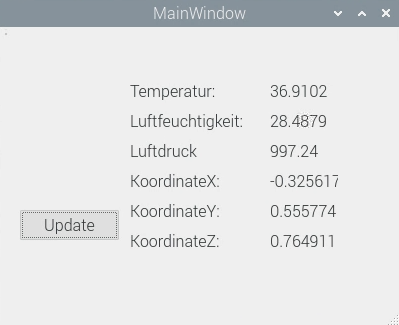
\includegraphics[width=0.55\textwidth, center]{StandDerTechnik/QtGUI}
    \caption[GUI der beispielhaften Anwendung]{GUI der beispielhaften Anwendung}
    \label{img:qtGui}
\end{figure}
